\documentclass{article}

\usepackage{graphicx} % Required for the inclusion of images
\usepackage{amsmath} % Required for some math elements
\usepackage{graphicx} 
\usepackage[T1]{fontenc}
\usepackage[utf8]{inputenc}
\usepackage{lmodern}
\usepackage{float}
\usepackage{fullpage}
\usepackage{xcolor}
\usepackage[hidelinks]{hyperref}
\usepackage[bottom]{footmisc}
\usepackage{listings}
\usepackage{longtable}
\lstset{basicstyle=\fontfamily{fvm}\selectfont\footnotesize,
    showstringspaces=false,
    commentstyle=\color{red},
    keywordstyle=\color{blue}
}

\title{Effective House Energy Management Using Reinforcement Learning Technical Documentation} % Title

\author{Dawid Czarneta, Jakub Frąckiewicz, Filip Olszewski, Michał Popiel, Julia Szulc}

\date{\today}

\begin{document}

\maketitle

\begin{abstract}
This is a technical documentation of our university project developed with cooperation and guidance of Rafał Pilarczyk from SAMSUNG. Document contains a short introduction and overview of main concepts, milestones, goals and results of this project. It is followed by a technical part, that contains a setup guide, code and tests overviews, explanation of used algorithms and concepts. Last part provides details about the development process, including useful insights, experiences, further research suggestions and lessons we have learned the hard way.
\end{abstract}

\newpage
\tableofcontents
\newpage

\section{Introduction}
The idea of the project is to examine the potential of artificial intelligence in decision-making processes. This potential is based on the growing popularity of Reinforcement Learning systems, as well as amount of new research and successful results achieved by them. As those results are very often presented for either traditional or computer game environments (Chess, Go, Atari games) \cite{dqn_paper}, there is a natural intuition that these methods could present solid performance in the decision-making processes domain.


\subsection{Goals and milestones}
To follow the project's idea, the goal of the project was to introduce a Reinforcement Learning system for a smart house, which works properly under any user requirements and surrounding conditions and which results in visible energy saving. What we mean by this is that the smart house manager will be an RL agent with the access to the basic devices in the house as well as the inside and outside sensors. Agent should keep the parameters (temperature, light) close to user requested values, using the minimal amount of energy. The sensors collect the data (temperature, brightness and solar battery level) between the fixed time-frames. For each time-frame, goal is to make the most suiting decision, based on the requests and the collected data.

Performance of such system can give us some estimates about the current potential of Reinforcement Learning field, and the main question is: is it able to learn such tasks \textbf{at all}?

\subsection{Results}
The short and quick answer to questions stated above is yes, Reinforcement Learning methods can work as decision-making systems. We have implemented a realistic simulator of a house with controllable devices that can affect the inside temperature and light levels (currently these are: energy source, light level, window blinds, air conditioning and heater), as well as outside world part with simulated weather. We have built a self-learning algorithm, that through interaction with this environment can learn to satisfy requests with minimal energy consumption. Our project provides methods for learning new models with a lot of environment's and agent's parameters available, as well as a live simulation of a model managing the house and a manual testing feature to allow for more precise debugging of these modules.

In the next section we will provide technical details about the project and elaborate more on the results.


\begin{figure}[H]
    \begin{center}
        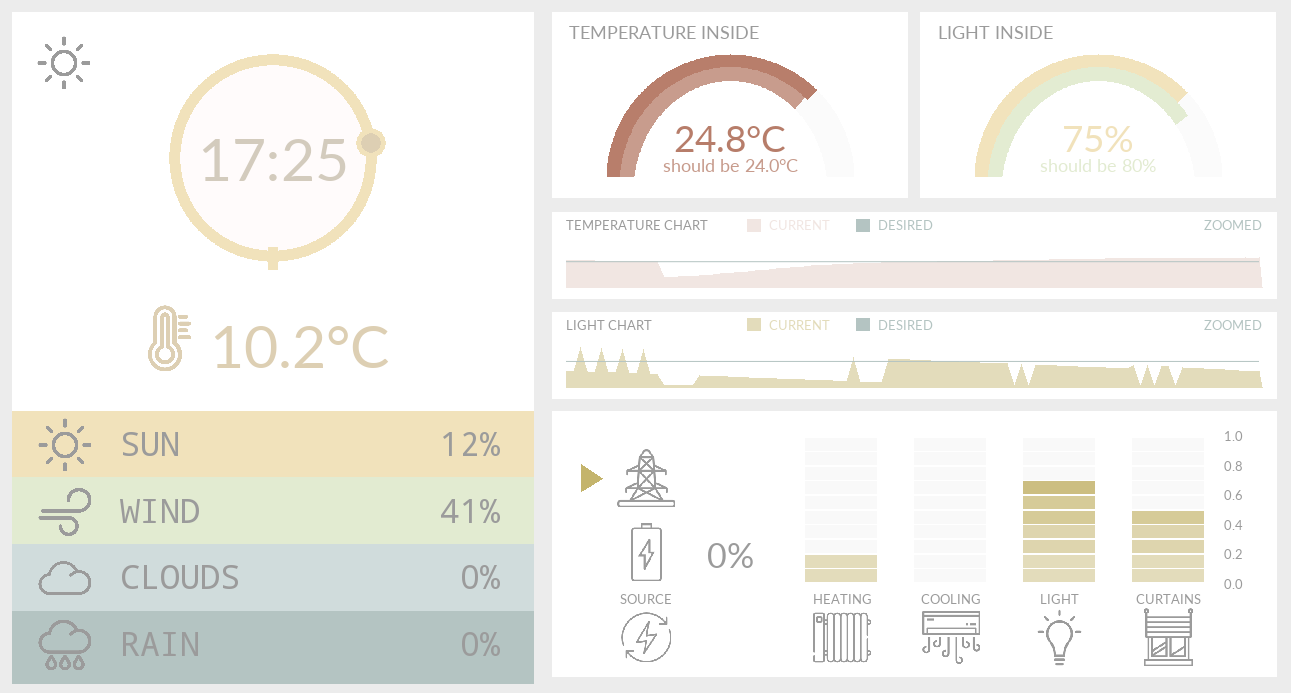
\includegraphics[scale=0.5]{screen.png}
        \caption{Screenshot from the simulation mode. Here, the user can see current time and information about \textbf{weather outside of the house} (on the left), current \textbf{house devices settings} (on the bottom right) and \textbf{last 100 readings of temperature and light} inside the house, in form of a chart (on the right center). Gauges on the top-right presents \textbf{current and desired level of temperature and light} respectively. The environment is changing dynamically - at every step, virtual \textit{agent} is making an action to control available devices in a way to optimize energy usage, while keeping in mind user's requests about temperature and light. More information about simulation can be found in section \textit{3.2 - Usage: Learning and Simulation}. 
        }
    \end{center}
\end{figure}

\section{Reinforcement Learning}
The project is based on one of the machine learning areas called Reinforcement Learning. The research and development of this field has been rising in recent years, because of, among others, the improvements in the deep learning methods and constantly increasing computing power that is available to human. Combined with concepts like convolutional neural networks, RL algorithms achieve super-human performance in a variety of tasks. The main field of success is probably the gaming world, including both the traditional games like Chess or Go, and computer games, where, for example, classic Atari games are learned and solved by RL agents taking the input directly from raw pixels \cite{dqn_paper}. Please note, that full explanation of the concepts - with fundamentals, equations and derivations - is not a goal of this documentation and we highly recommend to see the most well known sources (\cite{suttonBook}, \cite{silverCourse}) first.
\\\\
Reinforcement Learning is often explained by comparison to supervised learning, which is usually named the most successful field of Machine Learning. It is based on datasets, which consist of both the observations and the correct labels (answers, classes). For example, the dataset consists of images, and each image has it is correct label as well - a word that describes the object on the image. In Reinforcement Learning, on the other hand, there is no 'supervisor'. Instead, the environment returns a reward signal, which indicates how good or bad the current situation is. The main goal of the agent is to maximize the cumulative reward.
\\\\
There is a common vocabulary that is used to describe this setup. The \textbf{agent} (RL algorithm) has to interact with the \textbf{environment}, by performing \textbf{actions}. Environment gives the agent information about the \textbf{current state}, as well as the \textbf{reward signal} for the last time-frame. Agent has to choose the best one from the given set of possible actions. This is usually happening until the environment reaches a \textbf{terminal state}. Simulation from the start to terminal state is called an \textbf{episode}. A \textbf{transition} is defined as a sequence - state, action, reward and next state - and is used as a single 'experience' unit in agent's memory. 
\\\\
To put this into a perspective: In our project, the smart house manager is the agent. The simulated world is the environment. Actions are used to control devices such as heating or light. The state is a collection of information about the weather, inside parameters, current devices settings and user requests - everything that is needed for agent to perform rational decisions. The episode can be defined as - for example - one single day, where the terminal state is when the world clock reaches midnight.
\subsection{What have we used?}
Our agent uses Double DQN with Prioritized Experience Replay. This is a combination of recent developments in the field, which improve the speed, quality and stability of learning, and sometimes are essential for solving particular tasks. The neural network model is a fully connected feedforward network with one hidden layer. It uses ReLU activation function on hidden layer neurons and linear activation function on the output layer. For an explanation of these concepts and more detailed information about the agent, please see the Agent module section (4.2) and references at the end of the document.
\subsection{PyTorch Framework}
To implement the agent and the concepts named above, we have used the PyTorch framework \cite{pytorch}. It is now commonly believed, that this frameworks becomes the go-to Python framework used for Deep Learning, with some essential advantages when compared to the - currently most popular - TensorFlow framework. While this is still a matter of loud discussions, we have chosen the framework more out of curiosity, and because it is often called 'more Pythonic'. We will talk more about our experiences and conclusions about that choice later in the documentation, but the short story is - we are satisfied with it.
\\\\
We are using PyTorch for a very clear neural network model declaration, ready-to-use optimizers like SGD or Adagrad and loss functions, automatic computation of the gradients of network's parameters, and to perform the Double DQN learning process. It also provides a clear way to use GPUs for the computations. 

We have used the version 0.3.1 and it is important to note, that the newest stable version of the framework (0.4.0 on the day of this documentation's publication) requires some changes to the code.
\section{Getting Started}
\subsection{Setup and Requirements}
% Co zainstalować, jaka wersja Pythona, wszyściutko
This project was made on Debian based Linux distributions. We strongly 
recommend it in similar environment. 
\\\\
Firstly, install Python 3.6.5, python package manager and tkinter libraries. You can do it via apt package manager from command line
\begin{lstlisting}[language=bash]
$ sudo apt-get install python3.6 python3-pip python3-tk
\end{lstlisting}
or by downloading it from producent's page
\footnote{\url{https://www.python.org/downloads/release/python-365/}}
 and performing manual installation.
\\ \\ 
Secondly, go to main project directory and install required Python libraries:
\begin{lstlisting}[language=bash]
$ pip3 install -r requirements.txt
\end{lstlisting}
From now on, you should be able to use our project by running different source scripts.

\subsection{Usage: Learning and Simulation}
% Tutaj opis możliwych trybów uruchomienia. Main/learning na start, potem symulacja. Zaznaczyć już tutaj istotność configuration.json itd.
Our project can be run in different modes. These can be configured by changing contents of 
\textbf{configuration.json} file, located in main project directory. This directory will be referred to as 
\textbf{TOP} in this section. 

\subsubsection{Learning mode}
This mode can be run by going into source files directory and launching \textbf{main.py}
 with python3 interpreter. 
\begin{lstlisting} 
$ cd TOP/src
$ python3 main.py
\end{lstlisting}
In learning mode, Reinforcement Learning Agent model is learning for a given number of episodes.
One episode is typically one day in randomly generated environment. Agent is performing action every few minutes, trying to get perfect balance between required conditions (light, temperature) and energy cost; he is also drawing conslusions from his mistakes. As the time passes, Agent is getting better; we can roughly say
that in the long term, a longer trained Agent will perform better than the one after shorter training session,
with the same training configuration.
\\\\
After training session, model is typically saved in
\begin{lstlisting}
$ TOP/src/saved_models/
\end{lstlisting}
directory, within a separate folder with new index (indexes start at 0). Model is saved along with its configuration file, graph presenting learning curve and log with rewards from every step.
\\\\
Existing agent model can also be loaded into training session. In this case, you will be prompted to insert existing model's index number. Important to note here is that loaded model's parameters will be set from it's specific configuration file from it's folder, and the rest of the configuration (environment, main) will be loaded from the general configuration file.
\\\\ 
Basic configuration for this mode can be modified by changing contents of configuration.json, a part called \textbf{main}. Precise documentation of the whole configuration file can be found later in documentation. 
\\\\
\textit{NOTE:} Altough basic configuration for main (learning) mode is fairly limited, succesfull learning is built upon all environment / agent settings in configuration file. Default ones are based on our research in order to provide the best and most meaningful learning results.

\subsubsection{Simulation mode}
This mode can be run by going into source files directory and launching \textbf{simulation.py}
 with python3 interpreter. 
\begin{lstlisting}
$ cd TOP/src
$ python3 simulation.py
\end{lstlisting}
After launching, you will be prompted to insert existing model's number to use in simulation. 
\\\\
\textit{NOTE:} Simulation will start in full screen, be sure to have only one monitor connected - otherwise, simulation will span across all monitors.
\\\\
In simulation mode, user is presented to graphical interface representing Reinforcement Learning
Agent in action. 
There is a continuous environment, inside which Agent is trying to make his best decisions. No
learning process included.  \\\\
\textbf{Key mapping scheme}: \\
\begin{center}
{\def\arraystretch{1.3}\tabcolsep=10pt
\begin{tabular}{c | c }
\textbf{key} & \textbf{action} \\ \hline
ESC & exit simulation \\ \hline
SPACEBAR & toggle pause / play \\ \hline
- & slow down simulation \\ \hline
= & speed up simulation \\ \hline
z & toggle charts zoom \\ 
\end{tabular}}
\end{center}
\textbf{Widgets}
\begin{itemize}
    \item Weather widget \\
    Located on the left side of the screen. This widget presents current time and weather informations outside of the house in form of a timer animation and five weather indicators: 
    \begin{itemize}
        \item temperature
        \item sun intensity
        \item wind intensity
        \item clouds intensity
        \item rain intensity
    \end{itemize}
    \item Devices widget \\
    Located on the right bottom of the screen. This widget presents current house devices settings. Those include:
    \begin{itemize}
       \item Energy source (icons) and battery level (percentage)
       \item Cooling, heating, light and curtains level (leveled bar chart) 
    \end{itemize}
    \item Charts widget \\
    Located on the right center of the screen. This widget presents last 100 levels of light / degrees of temperature inside the house, along with users required level at given time. \\\\
    These two charts can be zoomed by pressing ''z'' on the keyboard. Zooming centers chart in a way that required level is placed directly at half of the charts height and the visible range is between $-0.1 * max$ and $+0.1 * max$ for maximum light / temperature levels respectively.
    \item Gauges widget \\
    Located on the right top of the screen. This widget presents current and desired level of light / temperature in form of a gauge chart.
\end{itemize}

Default speed of simulation can be set in \textbf{configuration.json} file, in module ''simulation'', item ''fps''.

\subsection{Testing}
\subsubsection{Overview}
To make sure that the code is always consistent with the base objectives and works correctly, the unit tests has been implemented. All of them can be found in \textbf{src/tests/} directory. Besides the regular unit tests there is also a separate file containing code consistency tests.
	The agent model can be tested using simulation mode or, with accuracy of a single action, using manual testing mode which is described later.

\subsubsection{Coverage test}
There is also possibility to run a coverage test using Python Coverage.py tool. If the code coverage needs to be checked the commands need to be invoked as follows:
\begin{lstlisting}
$ cd TOP/src/tests
$ ./get_coverage.sh
\end{lstlisting}
The output is a .html file that can be found in htmlcov directory.

\subsubsection{Manual testing}
The project also includes a manual testing mode. It can be run by going into source files directory and launching \textbf{manual\_test.py} with python3 interpreter. 
\begin{lstlisting}
$ cd TOP/src
$ python3 manual_test.py
\end{lstlisting}
This mode is a command-line interface for manual testing of Reinforcement Learning Agent behavior. User can manually test agent-environment connection by deciding which action to make, or can load existing model to be able to ask for its choice in particular moment. The whole process is done one step at the time.\\
All actions are made by entering a number specific for a certain command. Commands and numbers are visible all the time on top of the rendered text. \\\\
Please note, that this mode was made mainly for testing purposes, and should be treated more as an additional tool in further development, than a project's functionality.
\newpage
\section{Code overview}
Below are the diagrams, descriptions of the fundamental parts of the project and informations about their implementation. 

\subsection{Class diagram}
\begin{figure}[H]
    \begin{center}
        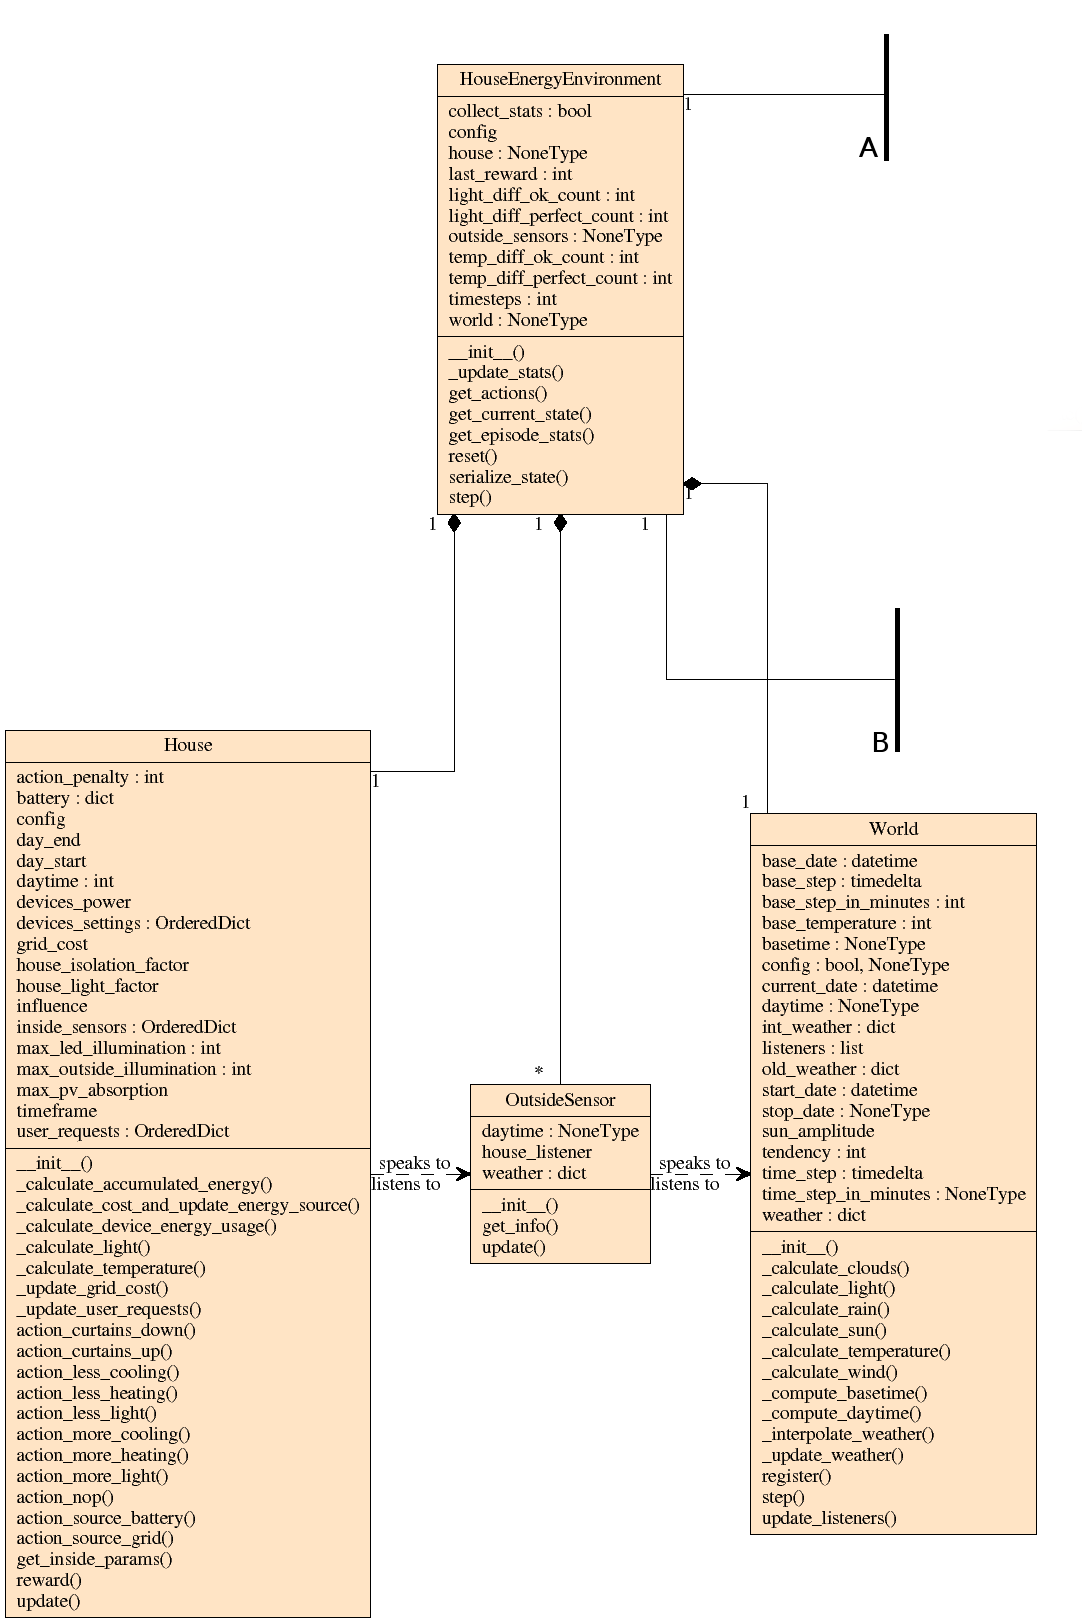
\includegraphics[scale=0.4]{classes1.png}
        \caption{First part of classes diagram}
    \end{center}
\end{figure}

\begin{figure}[H]
    \begin{center}
        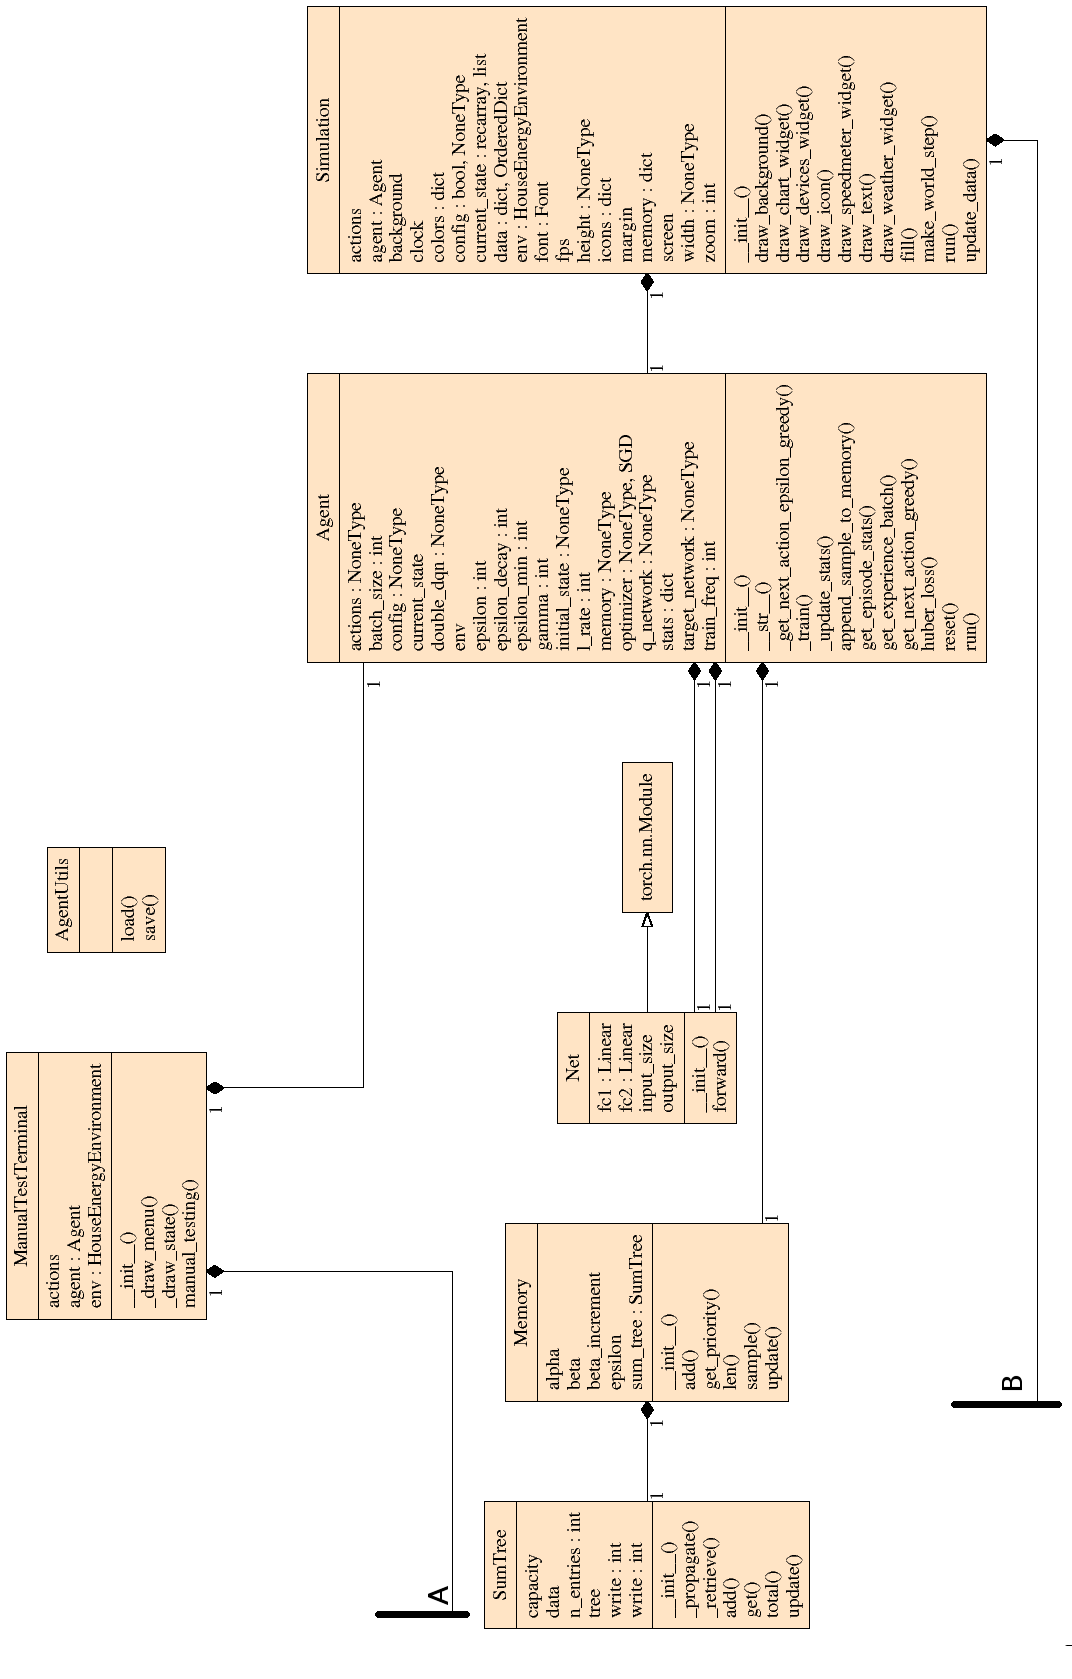
\includegraphics[scale=0.5]{classes2.png}
        \caption{Second part of classes diagram}
    \end{center}
\end{figure}

\begin{figure}[H]
    \begin{center}
        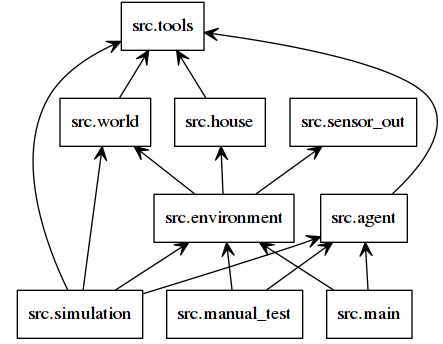
\includegraphics[scale=0.5]{packages.png}
        \caption{Modules diagram}
    \end{center}
\end{figure}

\subsection{HouseEnergyEnvironment module}
The environment where agent is put consists of a few separate classes that depend on each other and allow to create complex working setting that imitates the actual weather and the building.
\subsubsection{House}
This is where the agent is “placed” and where he operates. This class is responsible for generating the proper reaction after every time-frame, based on the agent’s action and outside world changes.

After each time-frame it receives the data from outside sensors and updates its parameters. During the update the temperature and light level are recalculated, energy cost increases and the energy stored in photovoltaics changes depending on the outside light and current energy source at home.

The House class contains a few methods used to calculate present environmental conditions. All of them implement the mechanisms that are meant to be as similar to the real world and its physics as possible. This way we could place the agent in the lifelike scenery and mimic its use in real life.

The vital part of the House is reward-calculating method. It is called after every time-frame. The important thing about the reward is the fact that it is always a negative value - that is why it can be treated as a “penalty”. The agent’s goal is to learn to minimize this penalty as much as possible. The reward formula is simply a weighted sum of penalties (temperature, light, energy cost) plus additional action penalty (for pointless or illogical actions like, for example, switching energy source to the one that is already used). 

As it can be seen in the source code of the House class, each action increases or decreases the given device setting by a constant, set in configuration, \textit{influence} value. We found it challenging to allow the agent to fully control the whole settings spectrum with single action, so to multi-task, it has to spread it's actions into multiple time-frames.

\subsubsection{World}
This class represents the model of the outside world. Its main purpose is to compute time and weather. Each time the method step is called, the world adds fixed time-frame value to the current time, updates weather and sends information about the changes to the listeners.

The weather changes are computed using the random values as well as fixed dependencies between specific components. Most of the weights and biases connected to weather were determined experimentally. The main goal was to provide natural-looking weather with varied rain periods, clouds, occasional storms etc.In order to achieve this, in some places a modified version of Gillbert-Elliot channel model was used to simulate constant periods of given weather phenomena.

\subsubsection{Environment}
Environment is indispensable part of the project. It connects smaller parts of the simulation like House and World into one working model. The class contains methods used to communicate with the agent as well as the ones that return human-readable information about current state. The central method in the agent-environment communication is the \textit{step} method and it was programmed to behave in a fashion known from \textit{OpenAI} gym environments. After the environment reached it's terminal state, the \textit{reset} method should be called before beginning a new episode. 

\subsection{Agent module}
The agent module is where all the Reinforcement Learning mechanisms are implemented and used. To get the idea of how to use it and how it works, we split the module into small components and explain each one by one.
\subsubsection{Neural Network}
The neural network model used in learning and choosing the actions is modeled as the \textbf{Net} class. It is fairly simple thanks to PyTorch framework and the code pretty much speaks for itself. The forward function defines the forward pass.

\subsubsection{Agent class}
The main class of the module is the Agent class and it is essential to know how to use this class. Most of the code is much more easier to read and understand with beginner knowledge in the RL field and fluency in writing PyTorch code. Here are the descriptions of the central methods of the class:

\begin{itemize}
\item \textit{reset()} - method used to reinitialize the agent. It is called from the constructor, but you can call it separately if there is a need.
\item \textit{run()} - most essential method, called to perform a full episode on the environment - with learning. This method resets the environment, and perform a loop in which the agent chooses an action, receives feedback, performs \textit{reward clipping}, updates statistics, saves the observed transition into the memory, calls the training function and then, in the end, slightly \textit{updates the target network}. The updates to the target networks are another concept that is used to stabilize the learning process and is explained in more detail in the next section.
\item \textit{learn()} - this is the method that performs training of agent's Q-network. It is a single training iteration, which samples a batch of transitions from memory and, based on Double DQN approach, performs the training on given batch. Training is explained in the next section. 
\item \textit{get\_next\_action\_greedy()} - returns next action given a state with use of the target network using a greedy policy. Greedy means that agent return the action with the biggest Q-function estimate. This function should be used if an outside object wants to know the agent's action for the given state.
\item \textit{get\_episode\_stats()} - method that implement the idea of collecting statistics about agent's actions, which is currently not used extensively. We are using these to register counts of each action to allow external object to analyze it.
\end{itemize}

\subsubsection{Double DQN}

The algorithm that stands behind the learning process and the so-called intelligence of our system is called Double DQN \cite{doubledqn_paper}. It is an extension to the basic Q-Learning algorithm. We fully recommend sources about these algorithms to understand the logic behind the algorithm (we placed the references to these sources at the end of the document), but we include a non-formal overview of the concepts with basic intuitions.
\\\\
\textbf{Q Function.} First, we need to understand what is the Q function and why the basic algorithm is based on learning this function to choose actions. Q function is a function of state and action to be taken in that state. Ideally, it is a value of the \textit{discounted cumulative reward} that the agent will receive, if it perform action a in state s, and then follow it's strategy to the end of the episode. Using the Bellmann equation, we can 'recursively' define this function, which is a very useful form later on:

\[ Q(S_{1}, A_{1}) = R_{1} + \gamma * (\max_{i} Q(S_{2}, A_{i}))\]

We want to learn our network to return the Q function values for all possible actions in the given state. So to construct an architecture which mirrors this behavior, the state is the input to the network, and each neuron in the output layer corresponds to one of the possible actions. We can clearly see, that - if we assume for a moment, that the network is fully learned - agent should always choose the action (neuron) with the highest Q value.
\\\\
\textbf{Q-Learning.} So this is how the agent chooses an action. But how to train the network? To be able to perform that, network has to know the errors for it's predictions. Q-Learning algorithm specifies how to calculate this error. What can be a surprise at first, we use the network itself to estimate that error. But is it not a magic trick - we introduce some real information that the agent received from the environment - the reward for the action it chosen. 
\\\\
To clear this up, the agent is in state $S_{1}$ and chooses an action $A_{1}$ with the best value $Q_{1}$, and the environment returns the reward $R_{1}$ for that action as well as the next state $S_{2}$. We use this feedback to perform an iteration of learning, using this formula to calculate the network's prediction error:

\[error = Q_{1}(S_{1}, A_{1}) - ( R_{1} + \gamma * (\max_{i} Q(S_{2}, A_{i})))\]

It is essential to see, that this algorithm uses the network itself to estimate the 'future' Q-function, but the learning is possible because of the reward information that comes from the observable environment - and this, in theory, leads the agent to the 'ground truth'. One more thing to mention - in the actual training, we use the loss function which combines errors calculated for each transition in the batch and returns a single number. To get the full understanding of the equation above, please follow sources linked at the end of the document. 
\\\\
\textbf{Q-Network and Target Network.} One of the improvements made to this setup is to split the network into two separate networks. One of the networks, Q-network, is the network that learns, and the second, target-network, is the one that makes action in the environment. The second one is slowly updated towards the q-network. This allows more stability to the agent - it explores the current strategy for some time before updating it's behavior for a new one. Agent that changes it's strategy after every step could be very noisy. Many approaches are used for the updates. We are using full updates each larger amount of steps, but also small updates after each step. This behavior can be controlled by configuration parameters.
\\\\
\textbf{DQN. \cite{dqn_paper}} Q-Learning can be performed with other function approximators, but the neural network version with mechanisms such as network splitting and Experience Replay (explained in the next section) is usually called DQN (short for DQN, the term was introduced by DeepMind in one of the well-known papers, it is listed in the sources section).
\\\\
\textbf{Double DQN. \cite{doubledqn_paper}} The Double DQN algorithm makes another improvement. It transforms the error formula a bit, making use of a separate network to deal with the positive bias introduced by the max operator. One of the tricks is to notice, that the second network (target network) can be used as that separate network to keep the split to 2, not 3 networks. This improvement is another one that is believed to stabilize the learning.
\\\\
\textbf{Epsilon Greedy Exploration.} Should agent always choose the best action? We see, that when first learning, the Q predictions are not really equivalent to the ground truth values. What is more - even if the network already learned a good strategy, maybe it should experiment and explore a bit to find an even better one? This is one of the key problems in Reinforcement Learning and the most usual way is to define the strategy of the action-making network as epsilon-greedy. What this means is that the network usually chooses the best action, but with \textit{epsilon} probability it chooses the action randomly. The epsilon starts with a big value to explore the environment heavily during the start - but it is decaying with each episode, allowing for precise optimization of the final strategy.
\\\\
\textbf{Reward Clipping.} Among some smaller things that are used in Reinforcement Learning to boost learning speed, agent uses reward clipping on the agent's side. One of the parameters in the configuration file sets the clipping value. In formal theory this is just better for the network learning process, because of the general normalization benefits, but in clear intuition, at some bad states it is not important \textit{how exactly bad is it} - but just that it is \textit{very} bad.

\subsubsection{Memory class}
One of the concepts that is essential for Deep Q Networks to work is the \textbf{experience replay}. Agent, instead of learning from sequence of observed, correlated transitions, saves them to a memory buffer and samples random transitions into a batch of uncorrelated ones. This improves stability of learning. It is still unclear what should be the perfect memory size, but it is proved that it matters. Another part of research tries to find out how to improve the sampling. Prioritized Experience Replay concept, where the transition is more likely to be chosen based on 'how wrong the network was about it', is reported to be a big improvement across many tasks.

Prioritized Experience Replay \cite{per_paper} was implemented by using a structure similar to a binary heap, called sum tree. The SumTree class can be found in the tools module, where we placed all context-independent logic of the project. It is an unsorted binary tree where the value of a node is a sum of its children. The leafs store transition's priorities and the root - total sum of all priorities. This approached is explained in more detail here \cite{dqn_per_post}.

\subsubsection{AgentUtils class}
This class provides methods for saving and loading the models of networks and configuration parameters. We have separated it from the Agent class for readability and file-based operations separate from the learning functionality of Agent class.

\subsection{Configuration file}
The project allows user to adjust values of some of the key parameters such as training settings or environment specifications. The whole list can be found in \textbf{configuration.json} file in the main project directory. All of the available parameters are listed below along with their types and brief descriptions.
{\def\arraystretch{1.2}\tabcolsep=5pt
\begin{longtable}{l|c|p{9cm}}
	\hline
	\textbf{Parameter name} & \textbf{Type} & \textbf{Description} \\
	\hline
    training\_episodes & integer & Number of episodes in training process.\\
    \hline
    save\_experiment & boolean & Determines whether the model has to be saved after learning.\\
    \hline
    save\_periodically & boolean & Determines whether the model should be saved each 1000 episodes, which gives an opportunity to see the evolving behavior of the model during learning.\\
    \hline
    print\_stats & boolean & Decides whether the episode statistics will be printed during the training. Statistics inform about most commonly taken action and percent of time in which the parameters where close to the requested values.\\
    \hline
    make\_total\_reward\_plot & boolean & Determines whether the plot of total episode rewards should be generated at the end of learning.\\
    \hline
    load\_agent\_model & boolean & Decides whether an already trained model should be loaded before training.\\
    \hline
    fps & integer & Number of frames per second in the simulation mode.\\
    \hline
    hidden\_layer\_size & integer & Size of the neural network hidden layer.\\
    \hline
    memory\_alpha & float & Agent's memory factor that determines how much prioritization will be used. (See 4.2.4 Section)\\
    \hline
    memory\_beta & float & Agent's memory parameter used in weighted importance sampling. (See 4.2.4 Section)\\
    \hline
    memory\_beta\_increment & float & The value by which the memory\_beta is gradually incremented during memory sampling. (See 4.2.4 Section)\\
    \hline
    memory\_epsilon & float & Agent's memory constant that prevents the transition from having a zero-valued priority. (See 4.2.4 Section)\\
    \hline
    memory\_size & integer & Size of the agent's memory.\\
    \hline
    double\_dqn & boolean & Determines whether DQN or Double DQN will  be used.\\
    \hline
    gamma & float & The discount factor in the DQN learning algorithm.\\
    \hline
    epsilon & float & Controls the exploration rate in the learning process (probability of choosing random action). We used the value greater than one to make sure that a couple of first episodes are fully random.\\
    \hline
    epsilon\_decay & float & The value by which the epsilon is gradually decremented after each episode.\\
    \hline
    epsilon\_min & float & The minimum value of epsilon.\\
    \hline
    batch\_size & integer & Size of transition batch retrieved from agent's memory for a training iteration.\\
    \hline
    learning\_rate & float & Value of learning rate in learning process.\\
    \hline
    training\_freq & integer & Defines the number of steps between subsequent train function calls, sometimes called 'frame skipping'.\\
    \hline
    target\_network\_update\_freq & integer & The frequency with which the target network is fully updated.\\
    \hline
    reward\_clip & integer & Value of parameter used in the reward clipping.\\
    \hline
    sgd\_momentum & float & Parameter used for network optimization by stochastic gradient descent with momentum.\\
    \hline
    q\_to\_target\_ratio & float & Proportion of q to target etwork weight update. \\
    \hline
    timestep\_in\_minutes & integer & Duration of single time-frame in the environment.\\
    \hline
    day\_start & integer & Number of minutes after midnight when the daytime begins.\\
    \hline
    day\_end & integer & Number of minutes after midnight when the nighttime begins.\\
    \hline
    devices\_power & integers & Power of the devices in the house (watt).\\
    \hline
    temperature\_w\_in\_reward & float & Weight of the temperature penalty in reward calculation.\\
    \hline
    light\_w\_in\_reward & float & Weight of the light penalty in reward calculation.\\
    \hline
    cost\_w\_in\_reward & float & Weight of the cost of the energy penalty in reward calculation.\\
    \hline
    max\_pv\_absorption & integer & Absorption of photovoltaic battery during the maximum sun intensity.\\
    \hline
    day\_grid\_cost & float & Grid energy price during the daytime.\\
    \hline
    night\_grid\_cost & float & Grid energy price during the nighttime.\\
    \hline
    house\_light\_factor & float & Determines how much of outside light is in the house.\\
    \hline
    house\_isolation\_factor & float & Parameter used in outdoor-to-indoor temperature calculation.\\
    \hline
    battery\_max & integer & Amount of energy in fully charged photovoltaic battery.\\
    \hline
    influence\_per\_min & float & Describes how large is the change of device setting when action is executed. Please note, that currently this is divided by two for light and curtains to provide better accuracy.\\
    \hline
    stats & floats & Values to be used for calculating 'ok' and 'perfect' percent of episode's time stats, calculated for temperature and light. 
\end{longtable}}

One of the tested configuration for which most of the models are actually learning the task pretty well is listed below. We were struggling to find a configuration, for which all of the launched models learned successfully. We address this issue to the exploration problem, as finding a strategy that compromises multiple goals can be a tough task. This is the configuration used for new models - because we have not implemented any learning rate decay and the epsilon\_min parameter is set pretty high, it is probably recommended to launch the learned agent for a 'tuning' phase of learning, with smaller learning rate and epsilon\_min, as this is the way to achieve the best of the best results. Please note, that the \textit{env} parameters are usually valued in the way that makes the simulator more realistic and probably should not be heavily changed. Exceptions are the penalty weights and devices power - while changes to the latter is probably not the cleanest way to change the agents behavior, the penalty weights can be used to place more impact on certain parameters. Tuning them turned out to be very tricky, but eventually we have found values that result in satisfying performances to the agent. We have found changes to the \textit{agent} parameters to make big yet unexpected changes to the learning quality. 

\begin{lstlisting}
{
    "main": {
        "training_episodes"          : 10000,
        "save_experiment"            : true,
        "save_periodically"          : true,
        "print_stats"                : true,
        "make_total_reward_plot"     : true,
        "load_agent_model"           : false
    },
    "simulation": {
        "fps"                        : 16
    },
    "agent": {
        "memory_alpha"               : 0.6,
        "memory_epsilon"             : 0.01,
        "memory_beta"                : 0.4,
        "memory_beta_increment"      : 0.001,
        "hidden_layer_size"          : 50,
        "memory_size"                : 30000,
        "double_dqn"                 : true,
        "gamma"                      : 0.95,
        "epsilon"                    : 1.1,
        "epsilon_decay"              : 0.9985,
        "epsilon_min"                : 0.1,
        "batch_size"                 : 16,
        "learning_rate"              : 0.0001,
        "training_freq"              : 4,
        "target_network_update_freq" : 500,
        "reward_clip"                : -2,
        "sgd_momentum"               : 0.95,
        "q_to_target_ratio"          : 0.02
    },
    "env": {
        "timestep_in_minutes"        : 1,
        "day_start"                  : 420,
        "day_end"                    : 1080,
        "devices_power": {
            "air_conditioner": 1500,
            "heater": 3000,
            "light": 720
        },

        "temperature_w_in_reward"    : 0.35,
        "light_w_in_reward"          : 0.82,
        "cost_w_in_reward"           : 0.024,
        "max_pv_absorption"          : 10,
        "day_grid_cost"              : 0.5,
        "night_grid_cost"            : 0.3,
        "house_light_factor"         : 0.0075,
        "house_isolation_factor"     : 0.996,
        "battery_max"                : 10000,
        "influence_per_min"          : 0.2,
        "stats": {
            "temp_ok_diff": 2,
            "temp_perfect_diff": 0.5,
            "light_ok_diff": 0.15,
            "light_perfect_diff": 0.05
        }
    }
}


\end{lstlisting}

\section{Accuracy measures}
\subsection{How to measure accuracy}
In machine learning, measuring model's accuracy, no matter what is the exact technique, is usually based on having some new, unseen data with correct labels and asking a model about it. In Reinforcement Learning we don't have the correct labels at all, the more complex the environment, the harder it is for human to prepare such unseen data by hand and determine the true correct answers. This problem is not that much of a trouble in gaming environments, because we can record some human total rewards and compare the learned model's score to an average person's score.
\\\\
For our environment, we came up with several possible measures during project's development. The first one was to use the \textbf{manual testing} script and inspecting single actions taken by agent in different conditions. While this was helpful in debugging and showing some environment inconsistencies, we could not easily express agent's performance that way. 
\\\\
The first solid accuracy measure is the \textbf{stats feature} that you can turn on as one of the configuration options. This feature registers the differences in actual and requested values of parameters, deciding whether the difference is too big, 'ok' or 'perfect', and sums it up as a percentage of time after the episode finishes. You can define exactly the difference values you find ok and perfect in the configuration file. For the values given in the example configuration in last section, we have found that for both light and temperature, a good agent can keep the differences 'ok' for the 90-100\% of the episode, and the 'perfect' differences for the 75-90\% of the episode. These values differ a lot with each episode, because of the changes in requests every 2 hours - some big changes can cause inevitable periods of too big differences, keeping these stats under the 100\% mark.
\\\\
Second way of performance measure is the \textbf{simulation mode}. It was built with a purpose of being a mode strictly for presentation purposes, but we quickly found out that this is a very good source of information about the agent. This mode, as described in the third section of the document, provides graphical widgets that show the current state of the environment and agent's actions. Graphs, even better when zoomed, can nicely present the tempo of adapting to new user requests. Any unwanted behavior will be quickly noticed. We highly recommend running every promising model through the simulation mode.
\\\\
We also recommend generating the total reward plots. These are useful to quickly see how the learning process looked and usually contains information about the stability and speed of learning. Also, reward plots that show a solid reward increase followed by a line that cannot go further up, suggest that the agent reached it's possible best performance. These models are then ready to investigate further with a simulation tool.  

\subsection{Impact of parameters on learning process}
Once the final version of the agent has been implemented, we have calibrated all of it's parameters in such a way that the agent's learning was as efficient as we could make it.
\\\\
Parameters were selected by repeatedly running new learning processes with differences in the configuration files. With limited computing power, it was hard to either come up with the very best configuration or to produce meaningful charts, analysis or conclusions about the impact of parameters.
\\\\
Even though, we still want to include a word or two about some of the parameters. We are assuming that there is no need to explain, how the parameters affect the speed of learning, because at this point, the reader should have some theoretical background about the way the Agent is working. 

\begin{itemize}
\item The network architecture should be kept as minimal as possible, and for this environment, one hidden layer was absolutely enough for the agent to learn a good strategy. We haven't found the minimal hidden layer size, but experiments suggest, that the value is below 60.

\item The memory size is an important parameter and should be tested a lot. There is some on-going research about making the memory size adaptive and it might be a good improvement to the current model. Also, it is known, that making the memory too small can cause instability, but too big memory can drastically slow down the training.

\item We did not notice any big improvements by introducing Double DQN, but it would need more tests to investigate properly.

\item We found that big exploration is one of the keys for founding a strategy that compromises many goals at once. We start with epsilon 1 (or higher than 1 for more fully-random episodes at the beginning) and use decays close to one (0.999 to 0.995). We also keep the epsilon\_min parameter pretty high, usually at 0.1. 

\item Another sensitive parameter is the batch size. We were using values between 8 and 16, and going outside of that interval never brought to us any promising results. Note that this parameter is somewhat correspondent to learning frequency, and if we set more steps between the training, the batch size should probably increase as well.

\item Learning rate could probably be changed some kind of scheduler to increase the final accuracies of the models. We use a constant one, and our successful models always used values smaller than 0.001.

\item A big leap forward was the introduction of momentum to our SGD optimizer. We were not able to train a single good model without momentum. We always kept the value high, between 0.8 to 0.95.

\item Parameters used for updating the target network need more tests, but we have not found them to make any noticeable impact.

\end{itemize}

\section{Development Process}
It is not a secret, that this project is more of a research than it is about making a production-ready system. While the most important research is concluded in the next section, we want to write couple of notes about our development process, to make it easier for new contributors to understand how the project was constructed. The most important tasks that were done are listed chronologically, and we also share some of the things that failed during the development process.
\subsection{Development Stages}
Here are the main stages of team's work during the project:
\begin{itemize}
\item Learning and research - learning about the Reinforcement Learning methods and algorithms - both the fundamental and specific ones that could fit to and solve the task, theoretical familiarization with the libraries and tools used in the next stages of system creation.
\item Planning - the stage in which the concept of the system was created with the initial schedule, class diagrams and division of roles between the team
\item Implementation of solutions - algorithms selected during planning has been implemented at this stage. This includes parameter tuning that finally led the agent to learn the task for the first time.
\item Improvement of the system - implementing extensions to the basic algorithm, optimizing the code and by performing another selection of parameters, the system has been improved in order to learn faster, perform better and have improved code-base readability.
\item System performance tests - the system has been tested to see if it behaves in the expected manner and to get some sense and conclusions about the speed, quality of learning, as well as impact of certain parameters.
\end{itemize}
\newpage
\subsection{Chronology}
Chronology of system preparation:
\begin{itemize}
\item Defining the organizational dates of such team meetings, talks with the project supervisor - 28/02/2018
\item Design the wireframe of application - 13/03/2018
\item The design of the reward function received by the agent - 13/03/2018
\item Creation of the class diagram - 15/03/2018
\item Implementation of actions possible to be performed by the agent - 19/03/2018
\item  Implementation of the reward function - 20/03/2018
\item  Agent class wireframe design - 25/03/2018
\item Preparation and implementation of internal dependencies - 24/03/2018
\item Preparation of a list of conventions on the source code of the application - 4.04.2018
\item Implementation of the basic version of the agent - 18/04/2018
\item Creation of weather dependencies in the environment - 18/04/2018
\item Documentation on the algorithms used in the agent - 19/04/2018
\item Manual tests of the environment - 20/04/2018
\item Saving and loading agent's neural network models - 25/04/2018
\item Analysis and tests of cloud solutions used to speed up calculations - 8/05/2018
\item Implementation of the console user interface - 8/05/2018
\item Implementation of Double DQN - 8/05/2018
\item Creation of configuration files for store Agent parameters - 14/05/2018
\item Design and functional requirements of the GUI - 4.05.2018
\item GUI implementation - 21/05/2018
\item Presentation of the system 11/06/2018
\end{itemize}
\subsection{What did not work out}
As a young team of developers, we are very happy to work on an exciting field of research, but we have to admit that some of the things about developing a solid, consistent code base for a team project turned out to be very challenging. Additionally, working with Reinforcement Learning agents and environments can be very tricky. In this section we are going to name some of the things that did not work out at all, including both our failures and concepts that have not improved the RL agent. 

\begin{itemize}
\item The first thing that we have failed in, is to maintain a full scalability of the environment. While there are some mechanisms that make it easier to add a feature to the simulator, like automatic action-methods detection, we feel that with more of an 'enterprise' approach to code architecture or more abstraction would make it even easier. The simulation and manual testing modes are designed more or less for the current state shape. The good news might be that the agent's class does not need any code tweaks during a state shape change.

\item We have not tried to compare the Q-Learning method with the other well known approach called Policy Gradient methods. These methods try to directly estimate the policy instead of Q function values, and, considering the characteristics of our environment, this could work even better. It might be harder to estimate a pretty complicated function, but fairly easy to find out about rules like 'turn heating on when it is too cold'. We list these methods as one of the possible further research suggestions.

\item One of the research fields in Reinforcement Learning is to allow development of RL environments to be easier by using a sparse reward function. This means that the agent receives a 0 signal, when the goal is achieved, and -1 otherwise. We have tried out this approach, using function similar to that described, and it drastically decreased performance of the agent. There are some recent improvements in the field, probably the loudest was the Hindsight Experience Replay concept, which was proven to, in some cases, condition the solving of a task, in which the reward function is sparse. We have not tried to implement this feature.

\item Another thing that made the learning process harder was the way we modeled the reward function at first. Both quadratic functions for penalties and concept of 'acceptance intervals' for light and temperature differences made the learning harder, as the resulting Q function, that our model had to estimate, got much more complicated that it needed to be. The lesson here was to keep the reward function simple, and to not introduce any constructs that might be rational to a human, but do no good for the agent. 

\item We have found that trying to perform learning computations on the GPU does not speed up the process. With a very simple neural network and small batch sizes, the overhead caused around 2 to 4 times slower execution of the learning mode. Please note that we were in possession of rather basic GPUs and newer, more expensive ones could potentially allow speed-ups.

\item While this might not be a proper failure, we are aware that the project - or this documentation - lacks statistics about the experiments, including results that would suggest the impact of certain parameters to quality of learning. We explain this by very broad space of possible configurations and limited computing power available during the development. It is also worth to come back to the project's main ideas and goals - as these were not strictly about extensive research on how to make the learning the fastest, but more to check the overall potential of Reinforcement Learning methods. 
\end{itemize}

\section{Conclusions}

This project has made it's initial goal of examining the potential of Reinforcement Learning in the context of decision-making processes, by training models that successfully manage a smart house environment, keeping the user requests fulfilled with optimized energy usage. We have developed a testing environment for new models and provided tools for both human-friendly simulations and low-level manual inspections of the inside transitions. Throughout the development process, we have learned a whole new machine learning field along with it's current research directions and reached several milestones, improving the simulator's realism and quality of models' learning processes. We have documented all the important information that we have encountered during the process. Our experience with this project suggests, that this field of research is very promising and exciting, yet still very hard to work with and a lot of concepts should be more heavily tested and investigated.
\subsection{Further Development}
Based on what we have not tried out yet and what have we read during the project development, we would like to list some of the potential improvements and further research directories.

\begin{itemize}
\item One of the obvious things that we recommend is to do a more exhaustive research, including series of multiple runs for the same configurations, to generate some aggregated, much more reliable and insightful statistics about parts and parameters of the project.

\item Extensions to the environment could, for example, introduce more outside factors, more 'extreme' conditions, more sensors or even a more complicated structure of the house. We think that is it not fully worth it to extend the state space, though. It already seems like neural networks can approximate strategies so well, that they can perform natural reasoning as long as the environment works reasonable.

\item The whole branch of Reinforcement Learning methods - Policy Gradients - are still an option to investigate and compare to the Q-learning method used here. 

\item The design of the network output layer, or more generally, environment's set of available actions, could be reconsidered. In given time-frame, agent can influence only one of the settings, only by increasing or decreasing the value by a constant. This setup is the only one that we could design successfully to not make the neural network's output layer to 'explode' in terms of size. This action space results in possible slow reactions to sudden user requirements changes. We found the current research and methods of continuous action spaces too challenging to understand and implement, but more experienced engineers could probably make some serious improvement to the current design.

\item There are some more improvements available to the Double DQN - Dueling DQN and Noisy DQN \cite{rainbow_paper} - and the current research yields some promising results that could be investigated in this project.

\item Goal-based Reinforcement Learning / Hindsight Experience Replay. Very new exciting research that was proved to enable solving particular robotics tasks with very sparse rewards, could be used (goal would be defined as the environment's user requests) to eliminate the reward function shaping, which could make the results even more impressive.

\item Adaptive memory size and experimenting with more of commonly used optimizers instead of SGD with Momentum - Adadelta, Adam. Gradient clipping. 

\item One of the team's ideas, that could extend the accuracy estimation, is to prepare a validation set of hand-shaped states in which the agent's correct answer would be \textit{obvious}, for example a state where the temperature parameter is perfectly set, but the light shines too bright. We have not prepared such a testing set, but this might be a way to extend the current testing method.

\item Totally separate, yet important suggestion is to bring the PyTorch code up to date with the changes made to the framework recently. Lot of code could be refactored due to the Tensors and Variables merge (now there are only Variables), new functionality that nicely substitute the usual CPU/GPU conditionals and more. 

\end{itemize}
\newpage

\begin{thebibliography}{99}

\bibitem{dqn_paper}
  \textit{Playing Atari with Deep Reinforcement Learning}: https://arxiv.org/abs/1312.5602

\bibitem{suttonBook}
  
  \textit{Introduction to Reinforcement Learning} from
  Richard S. Sutton and Andrew G. Barto: http://incompleteideas.net/book/the-book-2nd.html

\bibitem{silverCourse}
  \textit{Reinforcement Learning Course by David Silver}:
  http://www0.cs.ucl.ac.uk/staff/d.silver/web/Teaching.html 

\bibitem{doubledqn_paper}
  \textit{Deep Reinforcement Learning with Double Q-learning}: https://arxiv.org/abs/1509.06461
  
\bibitem{per_paper}
	\textit{Prioritized Experience Replay}: https://arxiv.org/abs/1509.06461
	
\bibitem{rainbow_paper}
  \textit{Rainbow: Combining Improvements in Deep Reinforcement Learning}: https://arxiv.org/abs/1710.02298
	
\bibitem{rl_repo}
	\textit{Reinforcement Learning - most popular repository of RL concepts implementation and exercises}: https://github.com/dennybritz/reinforcement-learning

\bibitem{dqn_per_post}
	\textit{Useful blog post with Double DQN and PER explained}: 
	https://jaromiru.com/2016/11/07/lets-make-a-dqn-double-learning-and-prioritized-experience-replay/

\bibitem{good_blog_post}
	\textit{Very useful post with a lot of insight and intuition about DQN, Double DQN and more}: http://neuro.cs.ut.ee/demystifying-deep-reinforcement-learning/
	
\bibitem{pytorch}
	\textit{PyTorch 0.3.1 Documentation}: https://pytorch.org/docs/0.3.1/

\end{thebibliography}

\end{document}

